\chapter{Fundamentos del lenguaje}
 
\section{¿Qué es MATLAB?}

MATLAB es un lenguaje de programación de alto nivel y entorno de
desarrollo interactivo, utilizado para numerosas aplicaciones de
carácter técnico y científicas. MATLAB permite realizar adquisición y
análisis de datos, desarrollo de algoritmos computacionales, creación y 
simulación de modelos físicos y la visualización gráfica de procesos 
determinados. Entre los campos de uso de MATLAB se incluyen el
procesamiento digital de señales, audio, imágenes y vídeo, sistemas de
control, finanzas computacionales, biología computacional, redes
neuronales, etc. \\

\emph{Características del lenguaje:} 

\begin{itemize}
\item
  \textbf{Interpretado:} Esta característica le convierte en un lenguaje no muy
  apto para aplicaciones donde la rapidez de ejecución sea crítica, pero
  esto mismo facilita la depuración de errores y permite un tiempo de
  desarrollo reducido en comparación a los lenguajes compilados
  tradicionales como C/C++.
\item
  \textbf{Tipado dinámico:} No es necesario declarar el tipo de variable a
  utilizar, MATLAB reconoce de forma automática el tipo de dato con el
  que trabajará, aunque claro que es posible declarar un tipo de dato de
  forma explícita utilizando las funciones de conversión adecuadas.
\item
  \textbf{Multiplataforma:} MATLAB está disponible para las plataformas más
  comunes: Unix, Windows, GNU/Linux y Mac OS.
\item
  \textbf{Multiparadigma:} Soporta programación imperativa, funcional y orientada
  a objetos.
\end{itemize}

\section{Descripción del entorno de desarrollo}

El entorno de MATLAB mostrado en la figura \ref{fig:screen_2012b}
pertenece a la versión 2012b, si dispone de otra versión quizá
encontrará cambios significativos en la interfaz, pero los componentes
más importantes permanecen invariables. \\

Como puede observarse en la figura \ref{fig:screen_2012b}, se
distinguen cuatro componentes en el escritorio del entorno MATLAB, los
cuáles son: \\

\textbf{Command Window} \\

Ventana de comandos interactiva en la cual deberán introducirse las
instrucciones de MATLAB, el prompt \verb|>>| le indica que está listo para 
recibir instrucciones. \\

\begin{informacion}{¿Qué es el prompt?}
En la jerga informática, se denomina prompt al símbolo o
caracter que aparece en una terminal o consola, cuando
esta se encuentra en disposición de aceptar un comando
de entrada.
\end{informacion}

\textbf{Current Folder} \\

Carpeta en la que se está situado, y en la que MATLAB buscará y guardará
(por defecto) los archivos generados durante la sesión. \\

\textbf{Workspace} \\

Ventana que muestra las variables creadas por el usuario durante la
sesión, indicando el nombre, valor y tipo de la misma. \\

\textbf{Command History} \\

Permite buscar comandos introducidos con anterioridad en la ventana de
comandos y ejecutarlos nuevamente o copiarlos. \\

\begin{center}
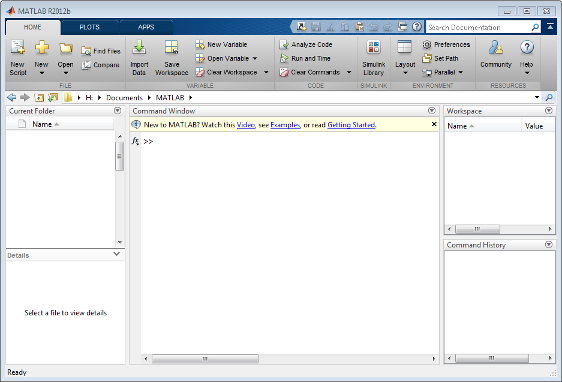
\includegraphics[width=0.8\textwidth]{src/img/ch1/img_1_1.png}
\captionof{figure}{Pantalla de MATLAB R2012b}
\label{fig:screen_2012b}
\end{center}

\section{Comandos básicos y generalidades}

\subsection{Consultar ayuda de MATLAB}

Uno de los puntos fuertes de MATLAB es la extensa documentación que
viene adjunta al software, la cual contiene múltiples ejemplos y
recomendaciones para la mayoría de las funciones. Puede acceder a la
ayuda ubicando el ícono característico de ayuda, o bien tecleando la
instrucción doc en la línea de comandos.\\

Si requiere una referencia rápida acerca de un comando o función puede
utilizar el comando \texttt{help} seguido por el nombre la función a
consultar, lo anterior le mostrará en la ventana de comandos una
descripción breve referente a la función consultada, por ejemplo la
siguiente línea le permite consultar ayuda rápida acerca del comando
\texttt{clc}:

\begin{matlab}
>> help clc
    clc    Clear command window.
    clc clears the command window and homes the cursor.
    See also home.
    Reference page in Help browser
    doc clc
\end{matlab}

\subsection{Limpiar ventana de comandos y variables del workspace}

Generalmente se considera una buena práctica de programación en MATLAB
iniciar los programas con instrucciones de limpiar la consola (Command
Window) y borrar las variables de la memoria. Lo anterior se logra
utilizando las instrucciones \texttt{clc} para limpiar la ventana de
comandos y \texttt{clear} para borrar las variables del workspace. Suele
acompañarse a la instrucción \texttt{clear} con el argumento adicional
\texttt{all}, que permite borrar incluso variables globales, es decir
conjuntamente: \texttt{clear all.}

\subsection{Líneas de comentarios}

Los comentarios de una sola línea en MATLAB deben comenzar con el
símbolo de porcentaje \%, todo aquello escrito después de este símbolo
será ignorado por el intérprete y reconocido como comentario,
asignándosele un color verde característico de forma automática.

\begin{matlab}
% Esto es un comentario en MATLAB
\end{matlab}

Para hacer bloques de comentarios (o comentarios multilínea) MATLAB dispone 
de una sintaxis específica que se muestra enseguida:

\begin{matlab}
%{
Esto es un comentario de múltiples
líneas en MATLAB, delimitado por 
llaves conjuntas con el signo % 
%}
\end{matlab}

\subsection{Valores especiales}\label{valores-especiales}

En la siguiente tabla se resumen algunos valores especiales
\emph{devueltos} por funciones predefinidas en MATLAB:

\begin{table}[h!]
\centering
% \rowcolors{1}{}{gray!20}
\begin{tabular}{p{3cm} p{12cm}}
\hline
\Centering\bfseries Función & \Centering\bfseries Descripción \\
\hline
\texttt{ans} & Guarda el ultimo valor no asignado a una variable \\
\texttt{eps} & Tolerancia que MATLAB soporta en los cálculos \\
\texttt{intmax} & Máximo valor entero que puede utilizarse \\
\texttt{intmin} & Mínimo valor entero que puede utilizarse \\
\texttt{realmax}  & Valor de coma flotante máximo que puede representarse \\
\texttt{realmin} & Valor de coma flotante mínimo que puede representarse \\
\texttt{pi} & Constante matemática (3.14159265…) \\
\texttt{inf} & Valor asignado a un número demasiado grande respecto a la
capacidad de cálculo del software. \\
\texttt{NaN} & Iniciales de “Not a Number”, tal cual traducción literal hace
referencia a un valor numérico inválido. \\
\texttt{computer} & Devuelve el tipo de computadora que se está utilizando\\
\texttt{version} & Devuelve la versión de MATLAB \\
\hline
\end{tabular}
\caption{Valores especiales}
\end{table}

\section{Tipos de datos y operadores}

El siguiente listado resume los tipos de datos más comunes en MATLAB:

\begin{itemize}
\item logical  (tipo booleano o lógico)
\item char (cadenas de caracteres)
\item numeric (datos tipo numérico)
\begin{itemize}
   \item int8, int16, int32, int64 (tipos entero)
   \item uint8, uint16, uint32, uint64  (enteros sin signo)
   \item single (flotantes de precisión simple)
   \item double  (flotantes de precisión doble)
\end{itemize}
\item cell (arreglos de celdas)
\item struct (estructuras)
\end{itemize}

\subsection{Tipo logical}

El tipo de dato lógico o booleano es en computación aquel que puede 
representar valores de lógica binaria, esto es 2 valores, valores 
que normalmente representan falso o verdadero. \\

En MATLAB las variables de tipo lógico permiten, evidentemente, dos valores, que
pueden ser \texttt{true} o \texttt{false}. Una forma de declarar una
variable de tipo lógico sería:

\begin{matlab}
>> a = true
a =
     1
\end{matlab}

Otra manera que resulta en lo mismo es la siguiente:

\begin{matlab}
>> a=logical(1)
a =
     1
\end{matlab}

Las líneas anteriores crean una variable \texttt{a} de tipo lógico con
un valor \texttt{true}. \\

La utilidad de los variables lógicas se hace evidente cuando es necesario 
tomar decisiones respecto al estatus o valor de una variable o subrutina.

\subsection{Tipo char}

Son cadenas de caracteres, que pueden contener valores alfanuméricos e
incluso símbolos especiales. Para declararlas no hace falta especificar
que son variables tipo \texttt{char}, dado que MATLAB es de tipado dinámico y
reconoce como tal aquellas cuyo valor asignado se encuentre delimitado
por comillas simples, un ejemplo muy clásico es el siguiente:

\begin{matlab}
>> txt = 'Hola Mundo'
txt =
Hola Mundo
\end{matlab}

El manejo de cadenas de caracteres o strings es una cuestión fundamental 
en la programación de computadoras. En MATLAB las cadenas de caracteres 
tienen muchas utilidades, entre las cuales pueden citarse: sirven como 
argumentos de entrada para funciones (como todo tipo de dato), identificadores 
para campos de estructuras, anotaciones y etiquetas en las gráficas, 
lectura y escritura de datos no uniformes, entre muchas otras. \\

En el capítulo 3 se aborda el manejo de strings de una manera muy completa, 
desde operaciones básicas como las comparaciones y concatenación, hasta el 
uso de expresiones regulares.

\subsection{Tipo numeric}

Normalmente cuando en MATLAB tecleamos un valor numérico o bien lo
asignamos a una determinada variable, esta será de tipo double, a menos
que se haga una conversión explicita a otro tipo de dato. Por ejemplo,
si insertamos en MATLAB lo siguiente:

\begin{matlab}
>> num = 10
num =
    10
\end{matlab}

Y posteriormente tecleamos la instrucción \texttt{whos} para verificar 
el tipo o clase de dicha variable:

\begin{matlab}
>> whos
  Name      Size            Bytes  Class     Attributes
  num       1x1                 8  double   
\end{matlab}

Si se requiere utilizar un dato de tipo entero habrá de realizarse la
conversión como sigue:

\begin{matlab}
>> numInt = int8(23)
numInt =
   23
>> whos
  Name        Size            Bytes  Class    Attributes
  numInt      1x1                 1  int8               
\end{matlab}

\subsection{Tipo cell}

Un cell array es un tipo de dato característico del lenguaje MATLAB que
consiste en un arreglo multidimensional de celdas que pueden contener
cualquier tipo de dato, inclusive otro cell array. Un ejemplo muy
sencillo de cell array se muestra enseguida:

\begin{matlab}
>> C={10,'MATLAB','5',[1 1]}
C = 
    [10]    'MATLAB'    '5'    [1x2 double]
\end{matlab}

\subsection{Tipo struct}\label{tipo-struct}

Las estructuras son arreglos de datos que, de forma similar a los cell
arrays, pueden almacenar variables de diversos tipos. Para la
organización de los datos se utilizan campos que pueden contener sólo un
tipo de dato. A continuación se muestra un ejemplo de cómo crear una
estructura:

\begin{matlab}
>> Alumno.Nombre='Jorge';
>> Alumno.Apellido='De Los Santos';
>> Alumno.Cursos={'Programación','Cálculo','Métodos Numéricos'};
>> Alumno.Notas=[10 9 10];
>> Alumno
Alumno = 
      Nombre: 'Jorge'
    Apellido: 'De Los Santos'
      Cursos: {'Programación'  'Cálculo'  'Métodos Numéricos'}
       Notas: [10 9 10]
\end{matlab}

En el capítulo 3 se tratan con más detenimiento las estructuras y su
utilidad en la programación en MATLAB.

\subsection{Referencias de función (function handle)}\label{referencias-de-funcion-function-handle}

Las \emph{function handle} son referencias asociadas a una función
nativa de MATLAB o bien a una función anónima creada por el usuario.\\

El siguiente ejemplo muestra la definición de una función anónima y su
posterior uso mediante su referencia:

\begin{matlab}
>> f=@(x) x+cos(x)
f = 
    @(x)x+cos(x)
>> whos
  Name      Size            Bytes  Class              Attributes
  f         1x1                32  function_handle              
>> fzero(f,0) % Raíz de la función 
ans =
   -0.7391
>> f(pi/2) % Evaluando función en un punto
ans =
    1.5708
\end{matlab}

\subsection{Identificar tipos de datos}

Para identificar tipos de datos en MATLAB se cuentan con diversos
comandos que nos facilitan esta tarea. El comando \texttt{whos} nos
proporciona información acerca de las variables existentes en el
workspace, tales como el nombre, tamaño y tipo. A manera de ejemplo
crearemos las siguientes variables e introducimos la instrucción whos
para verificar el tipo de información que nos imprime en la consola:

\begin{matlab}
>> n=10;
>> val=false;
>> s='MATLAB';
>> C={1,2,3};
>> ST.Nombre='Anna';
>> whos
  Name      Size            Bytes  Class      Attributes
  C         1x3               360  cell                 
  ST        1x1               184  struct               
  n         1x1                 8  double               
  s         1x6                12  char                 
  val       1x1                 1  logical      
 
\end{matlab}

Además del comando \texttt{whos}, puede utilizarse la función
\texttt{class} para determinar el tipo de dato de una variable pasada
como argumento, por ejemplo:

\begin{matlab}
>> a=3;
>> class(a)
ans =
double
\end{matlab}

\subsection{Conversiones entre tipos de datos}

Las conversiones entre tipos de datos son muy utilizadas en la
programación en cualquier lenguaje, puesto que permiten controlar la
precisión de los cálculos, mejorar la presentación de los datos o bien
evitar errores en la ejecución.

\subsubsection{Entre tipos numéricos}

Cuando se crea una variable de tipo numérico en MATLAB por defecto será
de tipo \texttt{double}, por ejemplo, creamos una variable llamada \texttt{num}:

\begin{matlab}
>> num=2;
>> class(num)
ans =
double
\end{matlab}

Las conversiones entre tipos numéricos son de sintaxis muy sencilla,
solo habrá que especificar el tipo de dato al cual se convertirá, siendo
permitidos los especificados en la tabla siguiente:

\begin{table}[h!]
\centering
% \rowcolors{1}{}{gray!20}
\begin{tabular}{p{5cm} >{\tt}P{5cm} p{5cm}}
\hline 
\Centering\bfseries Tipo de dato & \Centering\bfseries Sintaxis de conversión & \Centering\bfseries Rango \\
\hline
Precisión doble & double(num) & 2.2251e-308 a 1.7977e+308 \\
Precisión simple & single(num) & 1.1755e-38 a 3.4028e+38 \\
Entero de 8 bits & int8(num) & -128 a 127 \\
Entero de 16 bits & int16(num) & -32768 a 32767 \\
Entero de 32 bits & int32(num) & -231 a 231-1 \\
Entero de 64 bits & int64(num) & -263 a 263-1 \\
Entero sin signo de 8 bits & uint8(num) & 0 a 255 \\
Entero sin signo de 16 bits & uint16(num) & 0 a 65535 \\
Entero sin signo de 32 bits & uint32(num) & 0 a 4294967295 \\
Entero sin signo de 64 bits & uint64(num) & 0 a 18446744073709551615 \\
\hline
\end{tabular}
\caption{Conversiones entre tipos numéricos}
\end{table}

Así, podemos convertir la variable num, creada con anterioridad, a otro
tipo de dato numérico, por ejemplo a un entero de 8 bits:

\begin{matlab}
>> num=int8(num);
>> class(num)
ans =
int8
\end{matlab}

Es necesario poner especial atención en los rangos que pueden
manipularse con cada tipo numérico, debido a que por ejemplo si se
realiza la siguiente conversión:

\begin{matlab}
>> num=int8(653)
num =
  127
\end{matlab}

El valor que ha sido pasado como argumento de conversión excede el rango
para un entero de 8 bits, por lo cual simplemente se le asigna el máximo
valor permitido para una variable de este tipo. \\

Si requiere verificar por usted mismo los valores máximos y mínimos
permitidos para cada tipo de dato, puede usar las funciones
\texttt{realmin} y \texttt{realmax} para los tipos de coma flotante, y
las correspondientes \texttt{intmin} e \texttt{intmax} para tipos
enteros.

\subsubsection{De string a tipo numérico}

Para este tipo de conversiones MATLAB dispone de la funciones
\texttt{str2double} y \texttt{str2num}, en algunos casos no notará la
diferencia en los resultados, salvo en la rapidez de ejecución. Pese a
lo anterior, es necesario tomar en cuenta cómo trabaja cada función y
cual le resulta de utilidad; con \texttt{str2double} se convierte una
variable tipo string en un valor de tipo double, la función
\texttt{str2num} también realiza conversión a tipo double pero además
realiza conversiones a otros tipos de datos numéricos si se especifica
de manera explícita, de hecho esta tiene una funcionalidad muy similar a
la de la función \texttt{eval}. Los siguientes ejemplos muestran las
diferencias y utilidades de las funciones descritas.

\begin{matlab}
>> a=str2double('1237')
a =
        1237
>> b=str2num('1237')
b =
        1237
>> whos
  Name      Size            Bytes  Class     Attributes
  a         1x1                 8  double              
  b         1x1                 8  double     
\end{matlab}

\subsection{Operadores aritméticos, relacionales y lógicos}

Los operadores son símbolos especiales fundamentales en un lenguaje de
programación, se utilizan para \emph{operar} sobre variables
(operandos) y, de manera general, pueden clasificarse en tres grupos:

\begin{itemize} 
\item Operadores aritméticos
\item Operadores relacionales
\item Operadores lógicos
\end{itemize}

\subsubsection{Operadores aritméticos}

Los operadores aritméticos toman valores numéricos como entrada y
devuelven un valor resultante de aplicar la operación correspondiente
sobre los operandos. Por ejemplo, vea la siguiente expresión que
corresponde a una suma de escalares:

\begin{matlab}
>> 1+2
ans =
     3
\end{matlab}

En este caso \texttt{1} y \texttt{2} son los operandos o valores sobre
los cuales se aplica el operador \texttt{+}, y \texttt{3} es,
evidentemente, el resultado de ejecutar la operación. \\

En la siguiente tabla se listan los principales operadores aritméticos
disponibles en MATLAB.

\begin{table}[h!]
\centering
% \rowcolors{1}{}{gray!20}
\begin{tabular}{>{\tt}P{3cm} p{9cm}}
\hline
\normalfont\bfseries Operador  & \Centering\bfseries Descripción \\
\hline
+ & Operador  suma \\
- & Operador resta \\
* & Operador multiplicación (escalares) \\
/ & Operador división \\
./ & División elemento a elemento (matrices) \\
.* & Multiplicación elemento a elemento (matrices) \\
\hline
\end{tabular}
\caption{Operadores aritméticos}
\end{table}

Note que además de los operadores correspondientes a las operaciones
aritméticas básicas (suma, resta, multiplicación, división,
potenciación), se tiene operadores que realizan operaciones elemento a
elemento, que se utilizan para operar sobre arreglos matriciales.\\

Por ejemplo, sean \texttt{A} y \texttt{B} dos matrices de 3x3 definidas
como

$$
A = \begin{pmatrix}
1 & 2 \\
3 & 4 \\
\end{pmatrix}
\,\,\,\,\,\,\,\,\,\,\,\,
A = \begin{pmatrix}
5 & 6 \\
7 & 8 \\
\end{pmatrix}
$$

Si realizamos una suma o resta con estas matrices no habrá mayor
complicación, dado que tanto la suma y resta matricial se realizan
elemento a elemento:

\begin{matlab}
>> A=[1,2;3,4];
>> B=[5,6;7,8];
>> A+B
ans =
     6     8
    10    12
>> A-B
ans =
    -4    -4
    -4    -4
\end{matlab}

Luego, note las diferencias de utilizar la multiplicación elemento a
elemento (\texttt{.*}) y la ordinaria (\texttt{*}):

\begin{matlab}
>> A*B
ans =
    19    22
    43    50
>> A.*B
ans =
     5    12
    21    32
\end{matlab}

Sí, efectivamente los resultados son completamente diferentes: en el
primer caso se realiza una
\href{https://es.wikipedia.org/wiki/Multiplicaci\%C3\%B3n_de_matrices}{multiplicación
matricial}, siguiendo las reglas dictadas por el álgebra de matrices, en
el segundo caso lo que se hace es una multiplicación elemento a
elemento, es decir, cada elemento en la posición $(i,j)$ de
$\bf{A}$ se multiplica con el elemento ubicado en la misma
posición de $\bf{B}$.

\subsubsection{Operadores relacionales}\label{operadores-relacionales}

Los operadores relacionales se utilizan para comparar dos valores,
devolviendo un valor lógico. Normalmente se utilizan en conjunto con las
estructuras de control para la toma de decisiones sobre el procedimiento
o flujo de un programa.\\

La siguiente tabla resume los operadores relacionales: su notación y
descripción.

\begin{table}[h!]
\centering
% \rowcolors{1}{}{gray!20}
\begin{tabular}{P{3cm} p{4cm}}
\hline
\Centering\bfseries Operador  & \Centering\bfseries Descripción \\
\hline 
== & Igual a  \\
$<$ & Menor que \\
$>$ & Mayor que \\
$<$= & Menor o igual que \\
$>$= & Mayor o igual que \\
$\sim =$ & Diferente de \\
\hline
\end{tabular}
\caption{Operadores relacionales}
\end{table}

Puede ver que la notación difiere de la que ordinariamente utilizamos
cuando escribimos en papel, por ejemplo el símbolo del menor o igual
que $\le$ se escribe como \texttt{<=}. Es importante
notar que la comparación ``igual que'' se realiza con un doble signo
igual (\texttt{==}), puesto que el uso de un único signo corresponde a
la asignación, a continuación se muestra lo que ocurre cuando intentamos
hacer comparaciones utilizando sólo un signo \texttt{=}:

\begin{matlab}
>> 1==1
ans =
     1
>> 1=1
 1=1
 |
Error: The expression to the left of the equals sign is not a valid target for an assignment.
\end{matlab}

En el primer caso (doble signo) la comparación se hace devolviendo un
\texttt{true}, pero, en el segundo nos manda un error de sintaxis,
indicando que el \texttt{1} ubicado a la izquierda del signo igual no es
un caracter válido para realizar una asignación.

\subsubsection{Operadores lógicos}


\begin{table}[h!]
\centering
% \rowcolors{1}{}{gray!20}
\begin{tabular}{>{\tt}P{3cm} p{4cm}}
\hline
\normalfont\bfseries Operador  & \Centering\bfseries Descripción \\
\hline
\& & Operador lógico and \\
$|$ & Operador lógico or \\
$\sim$ & Operador lógico not \\
\hline
\end{tabular}
\caption{Operadores lógicos}
\end{table}

\section{Un mini tutorial de introducción}

Una vez conocidos los tipos de datos y los operadores, podemos comenzar
con una breve introducción al uso de MATLAB como una poderosa
calculadora muy fácil de utilizar, además vamos a ver algunas
características interesantes. Si hay algo en esta sección que te parece
díficil de asimilar, no debes preocuparte, lo subsiguiente se abordará
en capítulos posteriores de manera más \emph{detenida}.\\

Como se ha descrito en secciones anteriores, el command window o ventana
de comandos es la parte del entorno MATLAB que nos permite interactuar
de forma dinámica, si tecleamos una instrucción automáticamente nos
devolverá un resultado y se crearán variables en las cuales se almacenen
los diversos valores de salida. Por ejemplo, vamos a teclear una simple
suma aritmética:

\begin{matlab}
>> 3+2
ans =
     5
\end{matlab}

Puede verificar que en el workspace ahora aparece una variable llamada
\texttt{ans} con valor de 5, en \texttt{ans} se guarda por defecto el
último resultado no asignado a una variable, podríamos asignar el
resultado de la suma a una variable específica:

\begin{matlab}
>> suma=3+2
suma =
     5
\end{matlab}

Podemos también asignar valores a determinadas variables y enseguida
utilizarlas para ejecutar alguna operación, por ejemplo:

\begin{matlab}
>> a=5;
>> b=7;
>> a*b
ans =
    35
>> a-b
ans =
    -2
>> a/b
ans =
    0.7143
\end{matlab}

Note que el colocar un punto y coma (;) al final de una instrucción
evita que se muestre un resultado de salida, lo cual no afecta en el
almacenamiento de los valores correspondientes, pero podría resultar de
mucha ayuda al momento de seleccionar los valores que se quieren mostrar
en la ventana de comandos.\\

MATLAB también tiene disponible diversas funciones matemáticas
predefinidas, que pueden ser aplicadas sobre un número o sobre una
matriz o arreglo de números. Algunas funciones trigonométricas:

\begin{matlab}
>> sin(pi/2)
ans =
     1
>> cos(pi/4)
ans =
    0.7071
>> tan(pi/3)
ans =
    1.7321
\end{matlab}

Note que el valor de la constante $\pi$ está predefinida en
MATLAB mediante la cadena \texttt{pi}:

\begin{matlab}
>> pi
ans =
    3.1416
\end{matlab}

MATLAB devuelve un valor de 3.1416, lo cual es un valor
\emph{redondeado} de $\pi$, pero esto es cuestión solamente de
la representación, normalmente se utiliza el formato short (4 dígitos
después del punto decimal) para la representación de valores numéricos,
internamente MATLAB utiliza más digitos para \emph{manejar} y operar con
el valor de $\pi$. Si queremos obtener más digitos en la salida
por consola podemos cambiar el formato de salida:

\begin{matlab}
>> format long
>> pi
ans =
   3.141592653589793
\end{matlab}

El formato largo permite representar una cantidad con 16 decimales.
Incluso es posible \emph{forzar} a que se muestre una representación en
forma racional:

\begin{matlab}
>> format rat
>> pi
ans =
     355/113   
>> 0.1+0.123
ans =
     223/1000  
>> 0.125
ans =
       1/8
\end{matlab}

Se puede crear una lista o arreglo de valores numéricos encerrando estos
entre corchetes, y separando cada elemento por comas o espacios.

\begin{matlab}
>> A=[5,8,10,2,7]
A =
     5     8    10     2     7
>> B=[3 7 1 0 -2]
B =
     3     7     1     0    -2
\end{matlab}

Se puede obtener el valor máximo y mínimo de un arreglo numérico
utilizando las funciones \texttt{max} y \texttt{min} respectivamente.

\begin{matlab}
>> max(A)
ans =
    10
>> min(A)
ans =
     2
\end{matlab}

También podemos calcular el promedio de los valores utilizando la
función \texttt{mean}:

\begin{matlab}
>> mean(A)
ans =
    6.4000
\end{matlab}

Obtener la cantidad de elementos que componen lista con \texttt{length}
o \texttt{numel}:

\begin{matlab}
>> length(A)
ans =
     5
>> numel(A)
ans =
     5
\end{matlab}

Incluso podemos representar gráficamente cada uno de los elementos de un
vector mediante la función \texttt{plot}:

\begin{matlab}
>> x=[1,2,1,3,4,2,0,1];
>> plot(x);
\end{matlab}

\begin{center}
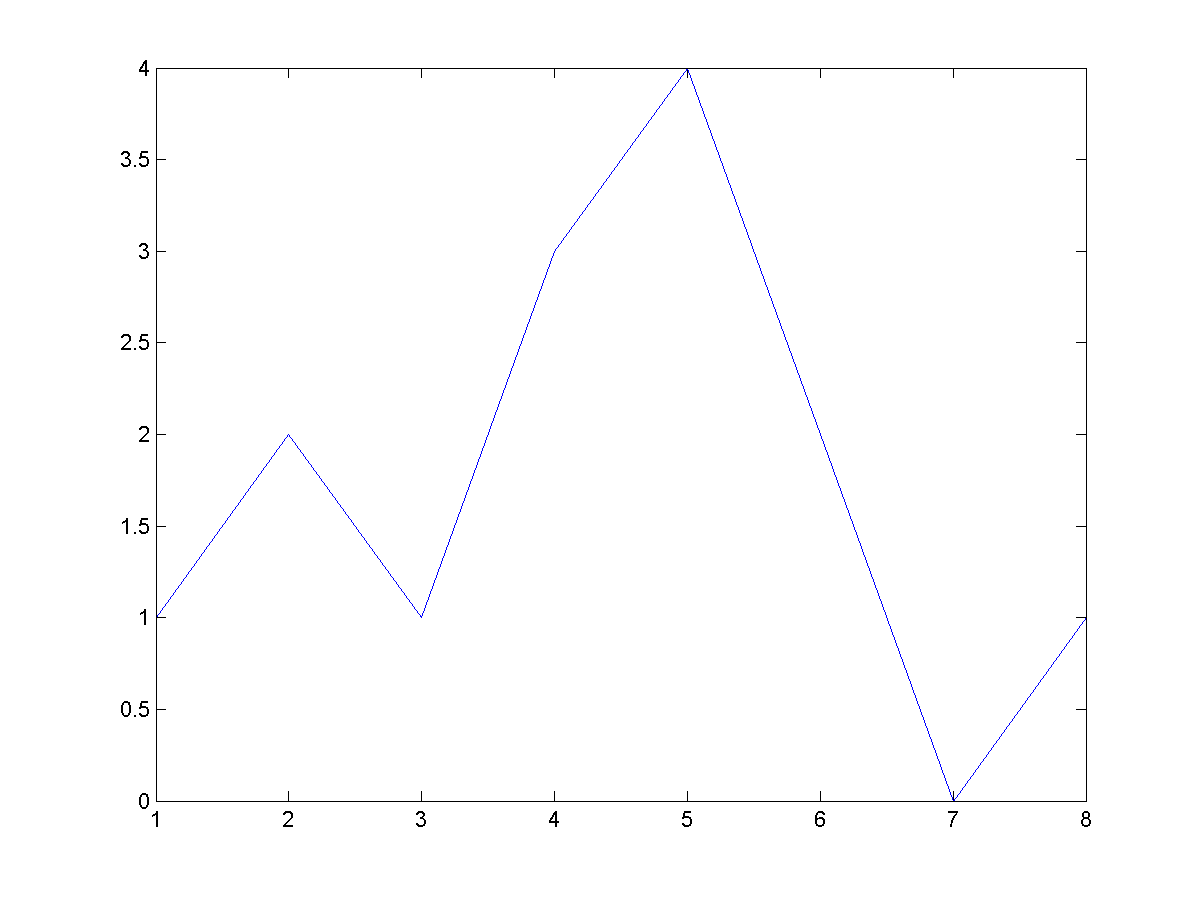
\includegraphics[width=0.6\textwidth]{src/img/ch1/img_1_2.png}
\captionof{figure}{Gráfica de un vector de puntos}
\label{fig:graph_fun}
\end{center}

De manera similar puede evaluar una función matemática en un intervalo
determinado y trazar su gráfica:

\begin{matlab}
>> x=0:0.01:10;
>> y=sin(x);
>> plot(x,y)
\end{matlab}

En lo anterior, se crea un vector \texttt{x} en el intervalo {[}0,10{]},
con incrementos de 0.01, es decir, el vector contiene los puntos:

$$ x = [0, 0.01, 0.02, 0.03,..., 9.99, 10] $$

Luego, al aplicar la función \texttt{sin} sobre ese vector, MATLAB
evalúa la función seno en cada uno de los puntos o valores contenidos en
el arreglo \texttt{x} y los guarda en \texttt{y}. El capítulo 2
(Vectores y matrices) trata con mayor profundidad la notación de dos
puntos utilizada y el manejo correcto de estructuras matriciales.

\begin{center}
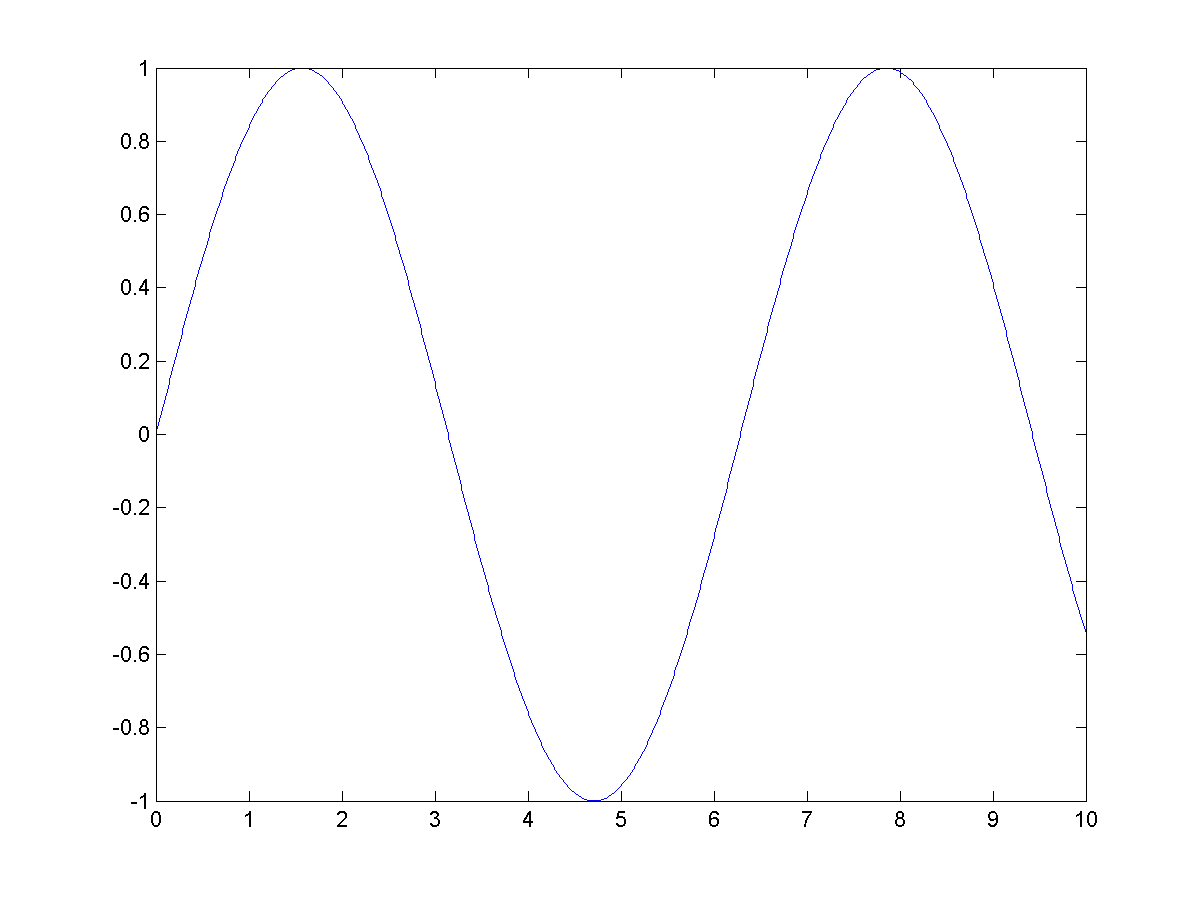
\includegraphics[width=0.6\textwidth]{src/img/ch1/img_1_3.png}
\captionof{figure}{Gráfica de la función $f(x)=\sin{x}$}
\label{fig:gla1}
\end{center}

¿Bastante interesante, verdad?. Bueno, incluso es posible trazar
gráficas de superficies tridimensionales con unas cuantas líneas de
código:

\begin{matlab}
>> [X,Y]=meshgrid(0:0.1:10, 0:0.1:10);
>> Z = sin(X)+cos(Y);
>> surf(X,Y,Z)
\end{matlab}

\begin{center}
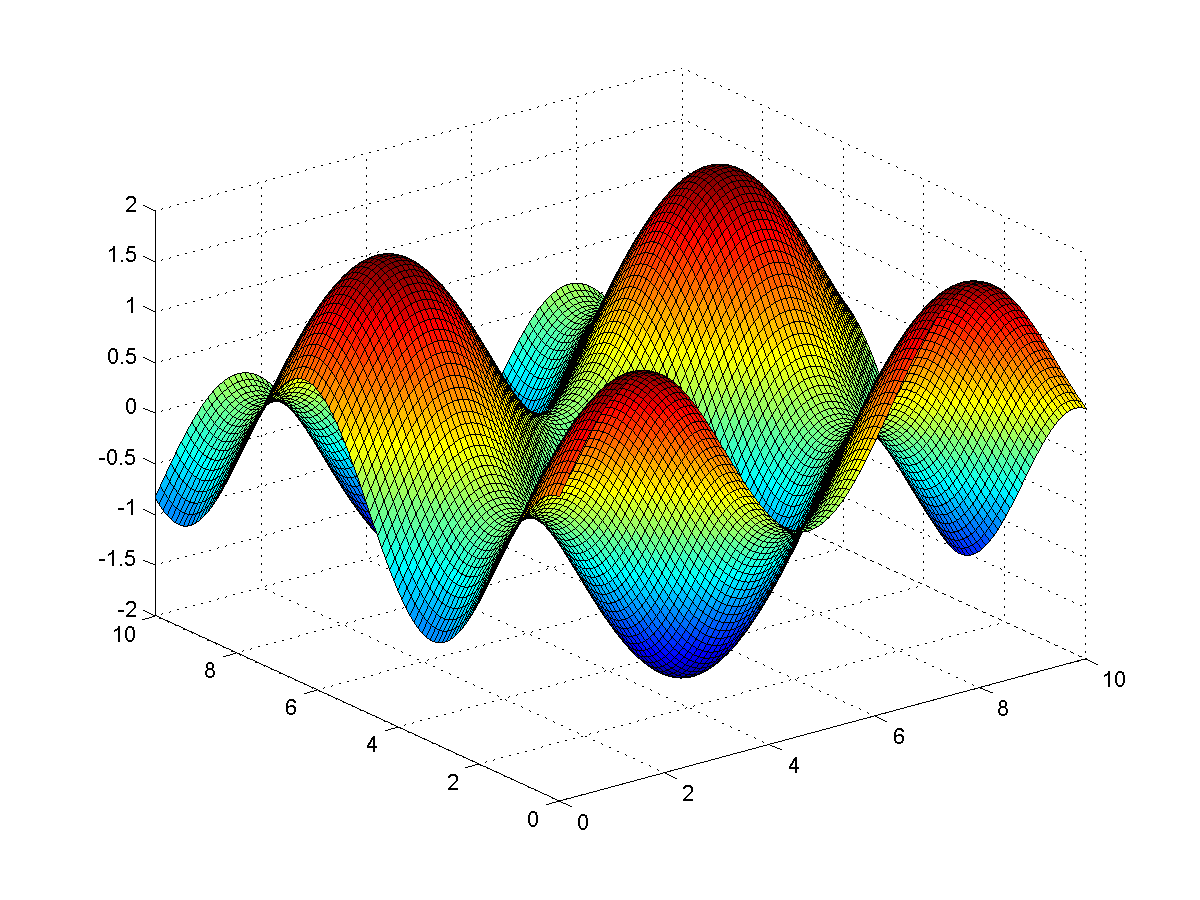
\includegraphics[width=0.6\textwidth]{src/img/ch1/img_1_4.png}
\captionof{figure}{Gráfica de una función $f(x,y)$}
\label{fig:xxxx}
\end{center}

Lo mismo podemos leer una imagen y hacerle algunos cambios
(restauración, segmentación, etc,...) utilizando el \emph{Image
Processing Toolbox} (que es una colección de códigos MATLAB que
facilitan esta tarea). Vea el siguiente ejemplo:

\begin{matlab}
>> img = imread('lena_std.tif');
>> img = rgb2gray(img);
>> filtro = [1 1 1; 1 -8 1; 1 1 1];
>> img_mod = imfilter(img, filtro);
>> imshow(255-img_mod)
\end{matlab}

\begin{center}

\includegraphics[width=0.4\textwidth]{src/img/ch1/lena.png}
\captionof{figure}{Imagen de Lena original}
\label{fig:lena}
\end{center}

\begin{center}

\includegraphics[width=0.4\textwidth]{src/img/ch1/lena_mod.png}
\captionof{figure}{Imagen de Lena modificada}
\label{fig:lena_mod}
\end{center}

Todo esto muestra un poco de lo que puede hacer MATLAB, pero, lo cierto
es que es un entorno muy completo con una \emph{infinidad} de opciones
que facilitan el desarrollo de algoritmos para aplicaciones en múltiples
disciplinas científicas. En los capítulos posteriores de este texto se
abordan algunas características y herramientas proporcionadas por MATLAB
para algunos campos específicos.

\section{Ficheros de comandos (scripts)}

Los ficheros de comandos, conocidos también como \emph{scripts}, son
archivos de texto sin formato (ASCII) con la extensión característica de
los archivos de MATLAB (*.m), se utilizan para almacenar una serie de
comandos o instrucciones que se ejecutan sucesivamente y que habrán de
realizar una tarea específica. Los scripts de MATLAB pueden editarse
utilizando cualquier editor de texto sin formato (Bloc de Notas,
Notepad++, Sublime Text, etc\ldots{}), aunque es más recomendable
utilizar el editor de MATLAB, puesto que proporciona herramientas que
facilitan la corrección de errores, el control sobre la ejecución del
código y la capacidad de autocompletado y sugerencias cuando se utilizan
funciones nativas de MATLAB.\\

Para crear un nuevo script puede pulsar la combinación \textbf{Ctrl + N}
(bajo SO Windows), o buscar en la interfaz de MATLAB la opción New y
enseguida seleccionar Script; si prefiere hacerlo desde la ventana de
comandos puede introducir el comando edit que le abrirá un nuevo script.\\

Para guardar un fichero de comandos utilice la opción \textbf{Save} de
la barra de herramientas o bien mediante la combinación de teclas
\textbf{Ctrl +S} en Windows. Debe tomarse en cuenta que al guardar un
script se le proporcione un nombre que no entre en conflicto con las
funciones nativas de MATLAB o las palabras reservadas del lenguaje.
Algunas recomendaciones que deben seguirse para nombrar un script son:

\begin{itemize}
\item
  El nombre deberá contener sólo letras, números o guiones bajos.
\item
  No deberá comenzar con un carácter diferente a una letra (Por ejemplo:
  \texttt{102metodo.m}, es un nombre inválido dado que comienza con un
  número).
\item
  Evite utilizar nombres de funciones nativas de MATLAB o palabras
  reservadas del lenguaje que podrían ocasionar conflictos.
\end{itemize}

Para saber cuáles son las palabras reservadas del lenguaje puede teclear
\texttt{iskeyword} en la ventana de comandos y MATLAB le devolverá un
cell array de strings:

\begin{matlab}
>> iskeyword
ans = 
    'break'
    'case'
    'catch'
    'classdef'
    'continue'
    'else'
    'elseif'
    'end'
    'for'
    'function'
    'global'
    'if'
    'otherwise'
    'parfor'
    'persistent'
    'return'
    'spmd'
    'switch'
    'try'
    'while'
\end{matlab}

Además, puede verificar si el nombre de un fichero existe utilizando la
función \texttt{exist}:

\begin{matlab}
>> exist('size')
ans =
     5
\end{matlab}

Si devuelve un resultado diferente de cero, entonces ese nombre está
siendo utilizado en una de las funciones/scripts incluidas en el path de
MATLAB.

\subsection{Ejecutando scripts}\label{ejecutando-scripts}

La utilidad de los scripts radica en la posibilidad de almacenar
comandos de manera estructurada y poderlos ejecutar posteriormente, para
hacerlo puede ir a la opción \textbf{Run} de la interfaz principal de
MATLAB y entonces se ejecutarán todas las intrucciones que conforman el
script.\\

Otra forma es ubicarse en la carpeta del script y teclear el nombre del
fichero en el Command Window. Claro que si el fichero no se encuentra en
el \emph{Current Folder} este no se ejecutará, exceptuando aquellos que
sean agreados al \emph{Path} de MATLAB. \\

\begin{informacion}{De los ficheros de funciones}
Para ejecutar los ficheros que contienen
definiciones de funciones no se procede como se ha
descrito anteriormente, puesto que, normalmente, estos 
necesitan \emph{información extra} o argumentos de entrada que deben
pasarse utilizando la sintaxis de \emph{llamada de
funciones}, misma que será objeto de estudio en
secciones posteriores.
\end{informacion}

\subsection{Modificando el Path de MATLAB}\label{modificando-el-path-de-matlab}

Primero, ¿qué es el path de MATLAB?, en resumen, son directorios o
carpetas en los cuales MATLAB \emph{busca} las funciones, clases y/o
ficheros en general que el usuario demanda durante una sesión.\\

Si teclea el comando \texttt{path}, este imprimirá en pantalla una lista
de directorios, ordenados de manera jerárquica, en los cuales MATLAB
busca las sentencias introducidas.\\

Por ejemplo, vamos a suponer que en nuestro directorio actual tenemos un
fichero llamado \texttt{principal.m} y que tenemos también una carpeta
\texttt{utils} en la cual tenemos algunos códigos necesarios
(\texttt{codigo1.m} y \texttt{codigo2.m}) para que nuestro código
principal funcione:

\begin{center}
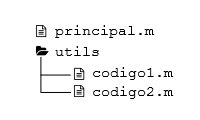
\includegraphics[width=0.3\textwidth]{src/img/ch1/path_example.pdf}
\end{center}

% \begin{verbatim}
% |
% └─── principal.m
% └─── utils
%         └─── codigo1.m
%         └─── codigo2.m
% \end{verbatim}

Una solución evidente (pero muy \emph{tosca}) es colocar los ficheros
\texttt{codigo1.m} y \texttt{codigo2.m} en el mismo directorio, pero
claro, eso implicaría tener muchos ficheros en una misma carpeta, lo
cual no suele ser buena idea.\\

Y la otra solución consiste en agregar la carpeta \texttt{utils} al path
de MATLAB, lo cual es tan sencillo como ejecutar:

\begin{matlab}
>> path(path, 'utils');
\end{matlab}

Con esto podrá llamar los ficheros \texttt{codigo1.m} y
\texttt{codigo2.m} desde \texttt{principal.m} sin necesidad de
colocarlos en la misma carpeta.

\section{Entradas y salidas en el Command Window}\label{entradas-y-salidas-en-el-command-window}

En la sección \ref{descripcion-del-entorno-de-desarrollo} se describió al Command Window (ventana de comandos) y
se hizo referencia a este como la parte del escritorio de MATLAB que
permite interactuar tecleando instrucciones y devolviendo al instante un
resultado. En esta sección veremos cómo utilizar funciones que permitan
introducir y mostrar ciertos valores de manera controlada por el
usuario.

\subsection{La función input}\label{la-funcion-input}

La función input permite \emph{pedir} un valor al usuario utilizando una
cadena de caracteres como prompt, la sintaxis es muy sencilla:

\begin{matlab}
var=input('Introduzca un valor: ');
\end{matlab}

En la variable var se guarda el valor que el usuario introduzca, los
valores aceptados por la función input pueden ser de tipo numérico, cell
arrays, e inclusive tipo char. Aunque para introducir cadenas de texto
la función input dispone de un modificador que hará que la entrada se
evalúe como una variable tipo char o cadena de texto, la sintaxis para
esto es la siguiente:

\begin{matlab}
var=input('Introduzca una cadena de texto: ', 's');
\end{matlab}

La letra s entre comillas simples le indica a MATLAB que deberá evaluar
la entrada como tipo string.

\subsection{Salida sin formato: la función disp}\label{salida-sin-formato-la-funcion-disp}

La función \texttt{disp} muestra en pantalla el valor de una determinada variable
que se pasa como argumento, por ejemplo:

\begin{matlab}
>> a=3;
>> disp(a)
     3
\end{matlab}

Para el caso anterior se pasa como argumento la variable a que ha sido
declarada previamente y simplemente se muestra el valor correspondiente
a esta. Las variables a mostrar pueden ser de cualquier tipo, incluyendo
cadenas de texto, matrices, cell arrays y estructuras, véanse los
siguientes ejemplos:

\begin{matlab}
>> disp(magic(3))
     8     1     6
     3     5     7
     4     9     2
>> disp({1,0,2,-2})
    [1]    [0]    [2]    [-2]
>> disp('Hola Mundo')
Hola Mundo
\end{matlab}

Con disp también es posible mostrar enlaces a un sitio web, utilizando
la sintaxis HTML para un enlace dentro de la función disp, por ejemplo:

\begin{verbatim}
>> disp('<a href="http://matlab-typ.blogspot.mx">MATLAB TYP</a>');
MATLAB TYP
\end{verbatim}

\subsection{La función fprintf}\label{la-funcion-fprintf}

Con \texttt{fprintf} es posible dar formato a la salida que se quiere
imprimir en pantalla, por ejemplo, es posible especificar el número de
decimales que se mostrarán o bien si se quiere mostrar como un entero o
quizá como una cadena de texto. La sintaxis de la función fprintf es
como sigue:

\begin{matlab}
fprintf('Especificaciones de formato',a1,...,an);
\end{matlab}

Donde las especificaciones de formato incluyen uno o más de los
identificadores de un mismo tipo o combinados que se muestran en la
siguiente tabla:

\begin{table}[h!]
\centering
% \rowcolors{1}{}{gray!20}
\begin{tabular}{P{4cm} p{7cm}} 
\hline
\bfseries Identificador & \Centering\bfseries Formato de salida \\
\hline
\texttt{\%d} & Tipo entero \\
\texttt{\%f} & Tipo coma flotante \\
\texttt{\%g} & Tipo coma flotante compacta. \\
\texttt{\%u} & Tipo entero sin signo \\
\texttt{\%e} & Tipo coma flotante, notación exponencial \\
\texttt{\%s} & Tipo char, cadena de texto \\
\texttt{\%c} & Tipo char, carácter a carácter.\\
\hline
\end{tabular}
\caption{Opciones de formato para \texttt{fprintf}}
\end{table}

Véase el siguiente ejemplo:

\begin{matlab}
>> fprintf('%d',pi);
3.141593e+00>>
\end{matlab}

Observe que se imprime el valor de $\pi$ en este caso, pero el
prompt de la ventana de comandos queda situado justo después del valor
de salida en la misma línea, para evitar lo anterior puede utilizar la
secuencia de escape \ver|\n| después del valor a
imprimir, lo cual le indica a MATLAB que debe comenzar en una nueva
línea. Modificamos y vemos el resultado que produce:

\begin{matlab}
>> fprintf('%d\n',pi);
3.141593e+00
\end{matlab}

Ahora observe lo que se imprime utilizando otros identificadores:

\begin{matlab}
>> fprintf('%f\n',pi);
3.141593
>> fprintf('%g\n',pi);
3.14159
>> fprintf('%e\n',pi);
3.141593e+00
>> fprintf('%u\n',pi);
3.141593e+00
\end{matlab}

Para las salidas de coma flotante puede especificar el número de
decimales que tendrá la salida, por ejemplo si desea mostrar solamente
dos decimales del número $\pi$:

\begin{matlab}
>> fprintf('%.2f\n',pi);
3.14
\end{matlab}

\section{Funciones}\label{funciones}

\subsection{Funciones, una introducción}\label{funciones-una-introduccion}

Las funciones son porciones de código que por lo general aceptan
argumentos o valores de entrada y devuelven un valor de salida. Una
función es una herramienta muy útil en la programación, dado que permite
la reutilización de código para procedimientos que lo requieran, así
como una facilidad significativa para mantener el código, lo cual se
traduce en una mayor productividad. MATLAB, de hecho, está compuesto por
una multitud de funciones agrupadas en \emph{toolboxs}, cada una de
ellas pensada para resolver una situación concreta.\\

Una función debe definirse en un fichero único, es decir, por cada
función creada debemos utilizar un archivo \texttt{*.m}, mismo que
tendrá el nombre dado a la función.\\

La estructura básica de una función contiene los siguientes elementos:

\begin{itemize}
\tightlist
\item
  La palabra reservada function
\item
  Los valores de salida
\item
  El nombre de la función
\item
  Los argumentos de entrada
\item
  Cuerpo de la función
\end{itemize}

Para una mejor comprensión de cada uno de esos elementos, refiérase a
las siguientes líneas de código:

\begin{matlab}
function res = suma(a,b)
res = a+b;
end
\end{matlab}

La función anterior llamada \texttt{suma}, recibe como argumentos de
entrada dos valores numéricos a y b, y devuelve un resultado guardado en
res que equivale a la suma aritmética de las variables de entrada. Note
que el valor de retorno debe asignarse a la variable indicada en la
línea de definición.\\

Si ejecutamos la función en la ventana de comandos obtenemos algo
similar a esto:

\begin{matlab}
>> s=suma(3,2)
s =
     5
\end{matlab}

Si no hace una asignación el resultado devuelto se guarda en la variable
\texttt{ans}.

\subsection{Verificar argumentos de entrada y salida}\label{verificar-argumentos-de-entrada-y-salida}

Cuando se crea una función es recomendable verificar si la cantidad de
argumentos de entrada corresponden a los soportados, o bien, si el tipo
de dato que se ha introducido es el adecuado para proceder con el resto
de la programación; MATLAB proporciona los comandos \texttt{nargin} y
\texttt{nargout} que sirven para \emph{contar} el número de argumentos
de entrada y salida respectivamente. \\

Utilizando como ejemplo la función suma creada con anterioridad, podemos
verificar que el número de argumentos sean exactamente dos para poder
proceder y en caso contrario enviar al usuario un mensaje de error en la
ventana de comandos, el código implicado sería similar al siguiente:

\begin{matlab}
function res = suma(a,b)
if nargin==2
    res=a+b;
else
    error('Introduzca dos argumentos de entrada');
end
end
\end{matlab}

Si ejecutamos la función pasándole solamente un argumento de entrada nos
devolverá un mensaje de error:

\begin{matlab}
>> s=suma(7)
Error using suma (line 5)
Introduzca dos argumentos de entrada
\end{matlab}

\subsection{Sub-funciones}\label{sub-funciones}

Las sub-funciones son funciones definidas dentro del espacio de otra
función principal. Se utilizan como funciones auxiliares con la
finalidad de hacer más legible el código y facilitar la depuración de
errores. Enseguida se muestra el ejemplo de una sub-función:

\begin{matlab}
function r=isfibo(num)
% Determina  si un  número  entero  forma  parte
% de la sucesión de Fibonacci, devuelve un valor
% de tipo lógico.
ff=fibonacci(num);
if any(ff==num)
    r=true;
else
    r=false;
end
    function F=fibonacci(n)
        F(1:2)=1;
        i=3;
        while 1
            F=[F F(i-1)+F(i-2)];
            if F(end) >= n,break,end;
            i=i+1;
        end
    end
end
\end{matlab}

La función anterior isfibo determina si el entero pasado como argumento
de entrada pertenece a la sucesión de Fibonacci, para ello utiliza como
una función auxiliar a la sub-función fibonacci que se encarga de
generar la sucesión de Fibonacci en un intervalo dado y guardarlo en un
vector de salida. Una sub-función puede ser llamada solamente por la
función principal que la contiene.

\subsection{Argumentos variables}\label{argumentos-variables}

En la introducción a las funciones se ha mencionado que estas por lo
general tienen un número específico de argumentos de entrada y salida,
no obstante se presentan situaciones en donde los argumentos de entrada
o salida de una función no son fijos o bien los argumentos pueden ser
demasiados de tal modo que resulte incómodo definirlos en la línea
correspondiente. Para solucionar lo anterior MATLAB permite el uso de
\texttt{varargin} y \texttt{varargout} como argumentos de entrada y salida
respectivamente. Para tener una idea más práctica de lo anterior véase
el ejemplo siguiente:

\begin{matlab}
function m=max2(varargin)
if nargin==1
    v=varargin{1};
    m=v(1);
    for i=2:length(v)
        if v(i)>m
            m=v(i);
        end
    end 
elseif nargin==2
    a=varargin{1};
    b=varargin{2};
    if a>b
        m=a;
    else
        m=b;
    end
end
end
\end{matlab}

La función anterior \texttt{max2} emula a la función nativa \texttt{max}, puede recibir
como argumento de entrada un vector o bien dos valores escalares. Si
observa el código anterior notará que varargin es un cell array que
guarda todos los argumentos de entrada pasados a la función, como se
verá en el capítulo 3 la manera de acceder a los elementos de un cell
array es utilizando la sintaxis: \texttt{var\{k\}}, donde \texttt{var}
es la variable en la que está almacenada el cell array y \texttt{k} es
el k-ésimo elemento contenido en el cell array.

\subsection{Ayuda de una función}\label{ayuda-de-una-funcion}

Como parte de las buenas prácticas de programación es recomendable
incluir comentarios dentro de una función que indiquen el propósito de
esta, así como una descripción breve de los argumentos de entrada y
salida e incluso un ejemplo concreto de la misma. \\

Por convención estos comentarios deben colocarse justamente después de
la definición de la función y antes de todo el código restante, además
de que esto servirá como referencia al resto de usuarios también le
permitirá a MATLAB interpretarlo como las líneas de ayuda cuando se le
solicite expresamente mediante la función help. Véase el siguiente
ejemplo:

\begin{matlab}
function [x1,x2]=ecuad(a,b,c)
% Resuelve una ecuación cuadrática de la forma:
% a*x^2+b*x+c=0
%
% Argumentos de entrada:
%          a  -  Coeficiente cuadrático
%          b  -  Coeficiente lineal
%          c  -  Coeficiente constante
%
% Argumentos de salida:
%          x1,x2  - Raíces de la ecuación cuadrática 
%
% Ejemplo:
%         >> [r1,r2]=ecuad(-1,2,1);
%
 
x1=(1/(2*a))*(-b+sqrt(b^2-4*a*c));
x2=(1/(2*a))*(-b-sqrt(b^2-4*a*c));
end
\end{matlab}

Podemos teclear help ecuad en la ventana de comandos y verificar lo que
MATLAB nos devuelve como ayuda de la función:

\begin{matlab}
>> help ecuad
  Resuelve una ecuación cuadrática de la forma:
  a*x^2+b*x+c=0
  Argumentos de entrada:
           a  -  Coeficiente cuadrático
           b  -  Coeficiente lineal
           c  -  Coeficiente constante
  Argumentos de salida:
           x1,x2  - Raíces de la ecuación cuadrática 
  Ejemplo:
          >> [r1,r2]=ecuad(-1,2,1);
\end{matlab}

Es común agregar a la ayuda de una función algunas referencias hacia
otras funciones similares, para ello en los comentarios debe agregar una
línea que comience con las palabras \texttt{SEE ALSO} (Ver también), seguidas
de las funciones similares separadas por comas, véase el ejemplo a
continuación:

\begin{matlab}
function [x1,x2]=ecuad(a,b,c)
% Resuelve una ecuación cuadrática de la forma:
% a*x^2+b*x+c=0
%
% Argumentos de entrada:
%          a  -  Coeficiente cuadrático
%          b  -  Coeficiente lineal
%          c  -  Coeficiente constante
%
% Argumentos de salida:
%          x1,x2  - Raíces de la ecuación cuadrática 
%
% Ejemplo:
%         >> [r1,r2]=ecuad(-1,2,1);
%
% SEE ALSO roots,solve,fzero
%
 
x1=(1/(2*a))*(-b+sqrt(b^2-4*a*c));
x2=(1/(2*a))*(-b-sqrt(b^2-4*a*c));
end

>> help ecuad
  Resuelve una ecuación cuadrática de la forma:
  a*x^2+b*x+c=0 
  Argumentos de entrada:
           a  -  Coeficiente cuadrático
           b  -  Coeficiente lineal
           c  -  Coeficiente constante
  Argumentos de salida:
           x1,x2  - Raíces de la ecuación cuadrática 
  Ejemplo:
          >> [r1,r2]=ecuad(-1,2,1);

  SEE ALSO roots,solve,fzero
\end{matlab}

\section{Bifurcaciones y bucles}

\subsection{Sentencia if-elseif-else}

La sentencia \texttt{if} se utiliza como bifurcación simple por sí sola,
es decir, en aquellas situaciones en las cuales se requiera evaluar
solamente una condición, por ejemplo, suponga que tiene dos números a y
b y necesita comprobar si son iguales y ejecutar una acción, para ello
bastaría con una sentencia \texttt{if} simple:

\begin{matlab}
if a==b
    disp('a es igual a b');
end
\end{matlab}

A diferencia del caso anterior hay situaciones que requieren la
ejecución de una acción cuando la condición se cumpla y de otra en caso
contrario, entonces puede utilizarse una bifurcación doble formada por
las sentencias \texttt{if-else}. Retomando el ejemplo para la
bifurcación \texttt{if} simple, podríamos modificarlo de tal manera que
envíe también un mensaje (ejecute una acción) para cuando la condición
no se cumple:

\begin{matlab}
if a==b
    disp('a es igual a b');
else
    disp('a es diferente de b');
end
\end{matlab}

Ahora imagine que para los ejemplos anteriores se necesita especificar
si a=b, si $a > b$ o bien si $a < b$, lo cual
implicaría tener una sentencia de selección múltiple
\texttt{if-elseif-else} que permite escoger entre varias opciones,
evaluándose en orden descendente, por ejemplo refiérase a la siguiente
estructura:

\begin{matlab}
if cond1
    % Instrucciones
elseif cond2 
    % Instrucciones
elseif cond3
    % Instrucciones
    .
    .
    .
elseif condN
    % Instrucciones
else
    % Instrucciones
end
\end{matlab}

MATLAB evalúa primeramente la condición 1 contenida en la sentencia
\texttt{if} (cond1) y en el caso de no cumplirse evalúa la siguiente
condición de forma sucesiva (cond2, cond3, ...); finalmente y en el
caso de que ninguna de las opciones evaluadas se cumpla, se ejecuta la
instrucción contenida en la sentencia else. A continuación se muestra el
ejemplo de una bifurcación múltiple para la situación descrita al
principio:

\begin{matlab}
if a==b
    disp('a es igual que b');
elseif a>b
    disp('a es mayor que b');
elseif a<b
    disp('a es menor que b');
end
\end{matlab}

\subsection{Sentencia switch}\label{sentencia-switch}

La sentencia switch es una bifurcación múltiple que permite seleccionar
entre varias opciones o casos la acción a ejecutar. La sintaxis general
es:

\begin{matlab}
switch var
   case opc1
      % Instrucciones
   case opc2
      % Instrucciones
    .
    .
    .
   otherwise
      % Intrucciones
end
\end{matlab}

Siendo var la variable que servirá como criterio de selección. Después
de la palabra reservada case, se coloca el valor de var para el cual se
ejecutarán esas instrucciones, y en otherwise se insertan las
instrucciones que MATLAB deberá ejecutar por defecto en caso de no
cumplirse ninguno de los casos especificados. \\

Enseguida se muestran dos ejemplos correspondientes a la sentencia de
selección switch:

\begin{matlab}
X=input('Inserte 0 o 1: ');
switch X
    case 0
        disp('Insertó cero');
    case 1
        disp('Insertó uno');
    otherwise
        warning('Valor incorrecto, verifique');     
end


letra=input('Inserte una letra: ','s');
switch letra
    case {'a','e','i','o','u'}
        disp('Es una vocal');
    otherwise
        disp('Es una consonante');
end
\end{matlab}

\subsection{Bucle for}\label{bucle-for}

La sintaxis general de un bucle for se muestra enseguida:

\begin{matlab}
for i=inicio:incremento:fin
    % Instrucciones...
end
\end{matlab}

El valor inicio es a partir del cual se ejecutará el ciclo, el
incremento es la cantidad que varía en cada paso de ejecución, y el
valor de final establece el último valor que tomará el ciclo.\\

El siguiente código muestra un ciclo for muy básico, el cual simplemente
muestra en consola el valor actual adquirido por la variable.

\begin{matlab}
for i=1:10
    fprintf('Valor actual: %g \n',i);
end
\end{matlab}

Cuando no se especifica el incremento, como el caso anterior, MATLAB
asume que es unitario.\\

Es posible utilizar ciclos for anidados, por ejemplo para cuando se
requiere recorrer una matriz en sus dos dimensiones y ejecutar
operaciones elemento por elemento. Véase el siguiente ejemplo:

\begin{matlab}
A=round(rand(5)*10);
for i=1:5
    for j=1:5
        disp(A(i,j));
    end
end
\end{matlab}

\subsection{Bucle while}\label{bucle-while}

El bucle while se utiliza, por lo general, cuando no se tiene un rango
definido sobre el cual se realice la ejecución del ciclo o bien cuando
la terminación del mismo viene dada por una condición. La sintaxis más
común es:

\begin{matlab}
while cond
    % Instrucciones
    % ...
    % ...
    % ...
end
\end{matlab}

Donde \texttt{cond} es la condición que determina la finalización de
ejecución. \\

Enseguida se muestra un ejemplo muy básico que muestra en pantalla el
valor de una variable utilizada como referencia:

\begin{matlab}
k=1;
while k<10
    disp(k);
    k=k+1;
end
\end{matlab}

Lo anterior muestra en consola el valor de k mientras esta sea menor a
10, es decir muestra todos los valores enteros en el intervalo
$[1,9]$, es importante notar que la variable k debe
incrementarse en cada ciclo para que en un momento determinado la
condición de finalización se cumpla, de lo contrario se convertiría en
un bucle infinito. \\

Ahora, veamos un ejemplo más práctico. La aproximación de una raíz
cuadrada por el método babilónico implica realizar n iteraciones
mediante la siguiente expresión:

$$ r_n(x) = \frac{1}{2} \left( \frac{x}{r_{n-1}}+r_{n-1} \right) $$

Donde x es el número del cual se calcula la raíz cuadrada. A
continuación se muestra el código implementado en MATLAB utilizando un
bucle \texttt{while}:

\begin{matlab}
x=input('Introduzca un número positivo: ');
r=x;
ra=0;
while ra~=r
    ra=r;
    r=(1/2)*(x/r+r);
end
fprintf('\nRaíz cuadrada de %g = %g\n\n',x,r);
\end{matlab}

Como se observa, en la variable ra se guarda la raíz aproximada
calculada en una iteración anterior, de manera que esta sirva como
comparación respecto a la nueva raíz calculada, el bucle termina cuando
la diferencia entre el valor actual y el anterior es inferior a la
tolerancia numérica (\texttt{eps}) soportada por MATLAB y por ende pasan
a considerarse como valores iguales. \\

\begin{informacion}{While-if-break, rompiendo ciclos.}
Es común utilizar el ciclo while poniendo un valor verdadero como condición, y 
usar la sentencia combinada \texttt{if-break} como punto de parada, por ejemplo:

\begin{matlab}
while true
    a = randi(10);
    if a>5
        break;
    end
end
\end{matlab}
\end{informacion}

\section{Fecha y hora}

Primeramente es importante mencionar que MATLAB maneja tres formatos de
fechas y hora, a saber:

\begin{itemize}
\item
  Un vector de seis elementos los cuales son: {[}año, mes, día, hora,
  minuto, segundo{]}.
\item
  Un valor escalar de coma flotante (tipo double), en el cual la parte
  entera representa la cantidad de días que han transcurrido desde el
  año cero (calendario gregoriano) y la parte decimal representa la
  fracción del día trascurrido.
\item
  Una cadena de texto con la forma \texttt{’dd-mmm-aaa\ HH:MM:SS’}.
\end{itemize}

Para obtener la fecha actual MATLAB proporciona el comando now:

\begin{matlab}
>> now
ans =
   7.3575e+05
\end{matlab}

Lo anterior podría resultar útil para efectos de cálculo pero no es tan
significativo para el usuario que está acostumbrado a visualizar la
fecha y hora mediante los formatos convencionales; podemos convertir el
valor numérico anterior a una cadena de texto que nos proporcione mayor
información a primer vista, para ello se utiliza la función datestr como
sigue:

\begin{matlab}
>> datestr(now)
ans =
03-Jun-2014 17:09:36
\end{matlab}

Además de las anteriores MATLAB dispone de las funciones datevec y
clock, la primera convierte una determinada fecha pasada como argumento
en formato string o numérico a un vector de seis elementos como se
describió anteriormente, y clock devuelve la fecha y hora actual tal
como la hace \texttt{now} pero como un vector de seis elementos. \\


\begin{ejemplo}{Ejemplo 1.1 Calculando área y perímetro de un círculo}
El área y perímetro (circunferencia) de un círculo vienen dados por las 
siguientes ecuaciones:

$$ A = \pi r^2 $$
$$ P = 2 \pi r $$

Escriba un programa que reciba como dato de entrada el radio del 
círculo y que imprima en consola el área y perímetro. \\

\textbf{Solución} \\

\begin{matlab}
r = input('Radio: ');
A = pi*r.^2;
P = 2*pi.*r;
fprintf('\nÁrea: %0.4f \nPerímetro: %0.4f \n\n',A,P);
\end{matlab}

Si ejecutamos el programa obtendremos algo como lo siguiente:

\begin{verbatim}
Radio: 5

Área: 78.5398 
Perímetro: 31.4159 
\end{verbatim}

\end{ejemplo} 

  \\  

\begin{ejemplo}{Ejemplo 1.2 Clasificando flujos}

El número de Reynolds es un parámetro adimensional utilizado en
mecánica de fluidos para caracterizar el movimiento de un fluido,
usualmente para un flujo interno en tuberías circulares se define como:

$$ Re=\frac{vD}{\nu} $$

Donde v es la velocidad del fluido, D el diámetro de la tubería a
través de la cual circula el fluido y $\nu$ la viscosidad cinemática.
La teoría subyacente del número de Reynolds se establece conforme a
varias características propias y externas al fluido, pero en este caso
vamos a limitarlo al flujo interno en tuberías circulares; siendo así,
el número de Reynolds permite caracterizar si un flujo es laminar o
turbulento dependiendo de ciertos intervalos establecidos de manera
experimental, enseguida se muestran los intervalos de valores y el
tipo de flujo en cada caso:

\begin{itemize}
\item Re $<$ 2100  \textit{Flujo laminar}
\item 2100 $\leq$ Re $\leq$ 3000   \textit{Flujo transitorio}
\item Re $>$ 3000   \textit{Flujo turbulento}
\end{itemize}

Basado en lo anterior, escriba un programa cuyos valores de entrada
sean la velocidad del fluido, el diámetro de la tubería y la
viscosidad cinemática, y que devuelva como variable de salida el tipo
de flujo.\\

\textbf{Solución:}

Vamos a implementar una solución utilizando la estructura de control 
\texttt{if-elseif-else}, en la cual nuestra variable o dato de comprobación 
será el número Reynolds.

\begin{matlab}
velocidad = input('Velocidad: ');
diametro = input('Diámetro: ');
viscosidad = input('Viscosidad: ');

Re = (velocidad*diametro)/(viscosidad);

if Re<2100
   disp('Flujo laminar');
elseif Re >= 2100 && Re <= 3000
   disp('Flujo transitorio');
else
   disp('Flujo turbulento');
end
\end{matlab}

¿Parece lo anterior una buena solución?.\\

Está muy bien, pero, y si alguien tiene la brillante idea de colocar 
cantidades negativas; el programa nunca se "quejará", pero desde luego estaremos 
entrando en una situación un tanto extraña, seguramente el programa nos mandará que 
estamos en el caso de un flujo turbulento, aún cuando los datos ingresados sean incorrectos.
Luego, lo que se quiere mostrar es que necesitamos trabajar más aún sobre ese código, 
asegurarnos que los datos ingresados sean los adecuados para realizar el cálculo. 
Claro está que en un código que necesitemos para nuestros deberes académicos pueda 
sonar un poco absurdo, pero en el mundo real estas cosas nunca, nunca están de más.
\end{ejemplo}

\section*{Problemas}

\textbf{1.1} ¿Qué tipo de dato devuelve cada una de las siguientes
instrucciones? (Puede verificar utilizando la función \texttt{class}).

\begin{matlab}
>> 3;
>> true;
>> 3==2;
>> {1,2,3}; 
\end{matlab}

\textbf{1.2} ¿Es posible realizar las siguientes operaciones?

\begin{matlab}
>> 3+int8(2);
>> true+5;
>> int8(10)+int16(5);
>> {1,2,3}+{0,1,0};
>> [5,1,-2]+[2 3 0];
\end{matlab}

\textbf{1.3} Desarrolle un script que le solicite su nombre (utilice la
función input) y que devuelva un saludo más el nombre ingresado, por
ejemplo: Hola Jorge, bienvenido. \\

\textbf{1.4} Identifique el error en las siguientes líneas de código:

\begin{matlab}
edad=input('Introduzca su edad: ','s');
if edad >= 18
    disp('Mayor de edad');
else
    disp('Menor de edad');
end
\end{matlab}

\textbf{1.5} Utilizando la escala de calificación del 0 a 10 y siendo 6
la calificación mínima aprobatoria, cree un programa en el cual ingrese
una calificación y este le devuelva un mensaje de APROBADO o NO APROBADO
en el caso que corresponda. \\

\textbf{1.6} El siguiente es un problema clásico en los cursos básicos
de programación: escriba un programa que determine si un número
ingresado es par o impar. \\

\textbf{1.7} Escriba una función llamada \texttt{sfibonacci}, que reciba
como argumento un entero positivo n, y que devuelva un vector con los
primeros n términos de la sucesión de Fibonacci. \\

\textbf{1.8} Desarrolle una función llamada \texttt{bucle\_test}, que
reciba como argumento de entrada un número entero N. Esta función debe
recorrer todos los valores enteros en el rango de 1 a N mostrando ``n es
divisible por 2'', ``n es divisible por 3'', ``n es divisible por 2 y
3'' o ``n no es divisible por 2 o 3'' (donde n será el valor actual).
Use un bucle for para recorrer los valores, la función \texttt{rem} para
verificar la divisibilidad y \texttt{num2str} para convertir cada número
en un string y mostrarlo en pantalla. Para verificar cada caso puede
utilizar una bifurcación múltiple \texttt{if-elseif-else}. 
\footnote{Danilo
  Šćepanović. 6.094 Introduction to MATLAB, January IAP 2010.
  (Massachusetts Institute of Technology: MIT OpenCourseWare),
  http://ocw.mit.edu (Accessed).} \\

\textbf{1.9} Escriba una función que le permita determinar si un número
entero pasado como argumento es primo, en caso de serlo devolverá un
valor lógico true y un valor false en caso contrario. (La función
\texttt{isprime} de MATLAB realiza la misma operación, pero claro, evite utilizarla 
en este caso).
